\documentclass{article}

\usepackage{geometry}
\usepackage{graphicx}
\usepackage{hyperref}
\hypersetup{
  colorlinks=true,
  linkcolor=blue,
  filecolor=magenta,      
  urlcolor=cyan,
  pdftitle={Overleaf Example},
  pdfpagemode=FullScreen,
}

\title{MIPS Assembly Assignment}

\author{
  Zakariyya Kurmally \\
  \texttt{2315839}
  \and
  Ihsaan Ramjanee \\
  \texttt{2315007}
}

\begin{document}

\maketitle

\pagebreak

\tableofcontents

\pagebreak

\section{Pseudocode}
\begin{center}
  \includegraphics[scale = 0.25]{ballspseudo.png}
\end{center}

% https://www.tutorialspoint.com/assembly_programming/pdf/assembly_basic_syntax.pdf
\section{The Code}
There are 2 main sections of code, the data and text section. The first
one is similar to preprocessor defines in C. They can be considered as
constants. The text part is where the most of the actual code is. 

\pagebreak

\subsection{Data Section}
\paragraph{}
The following contains all the constants and variables used throughout the 
program. 

\begin{center}
  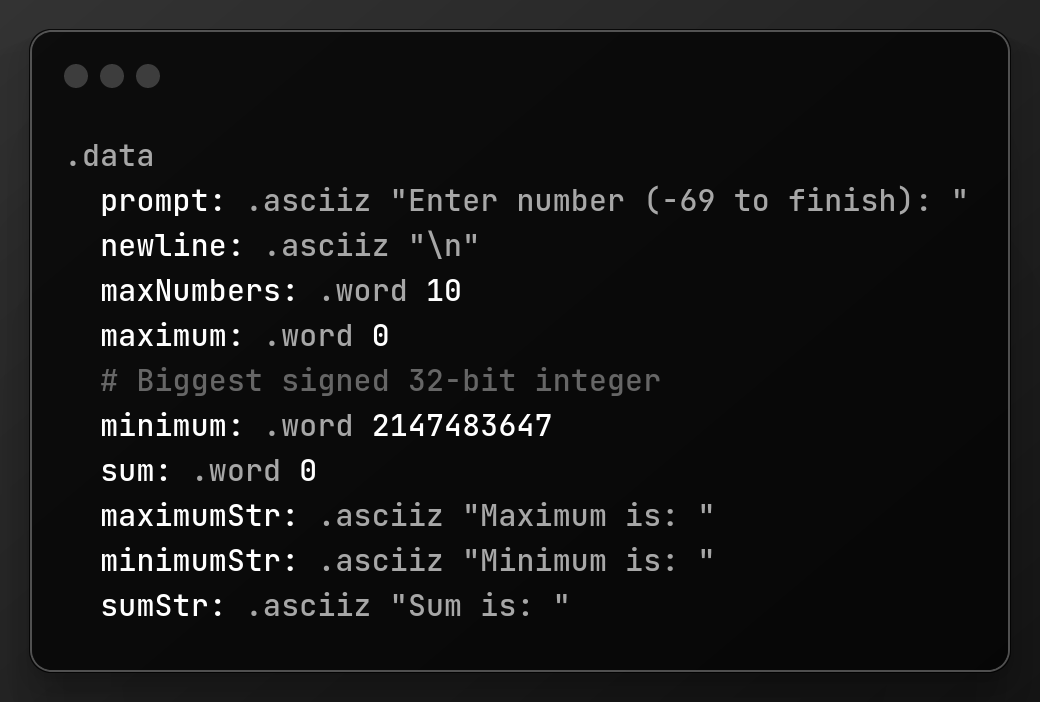
\includegraphics[scale = 0.25]{amen.png}
\end{center}

\subsection{Text Section}
\paragraph{}
We first initialised the pointer and counter variables:

\begin{center}
  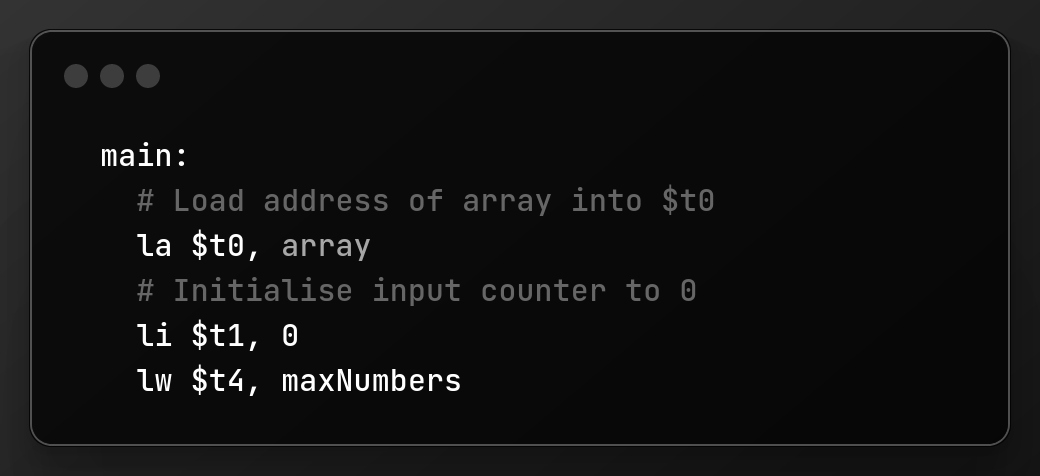
\includegraphics[scale = 0.25]{2nd.png}
\end{center}

Afterwards, the loop label takes over. It starts by prompting an input
from the user. After storing user input in \$t2, it compares it with a 
rogue value to see if the user want to stop. If that is not the
case, it will branch to the updateMaximum label if the new number
is greater than the current maximum. Finally, it will jump to
the checkMinimum label.

\begin{center}
  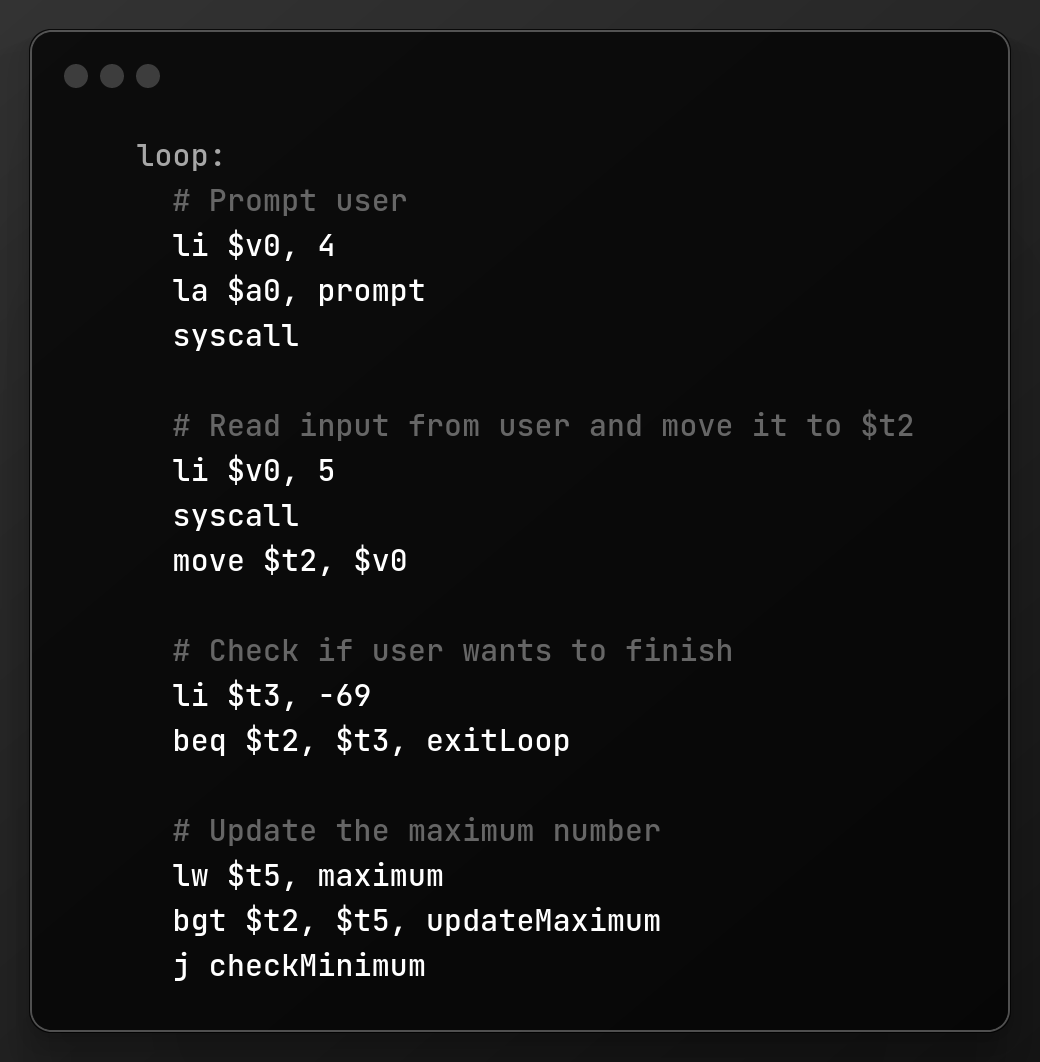
\includegraphics[scale = 0.25]{3rd.png}
\end{center}

The updateMaximum label stores the contents of the \$t2 register into
maximum and jumps to the checkMinimum label. The later will update the
current minimum, if need be, via the updateMinimum label. Otherwise,
it will jump to the sumAndLoop label.

\begin{center}
  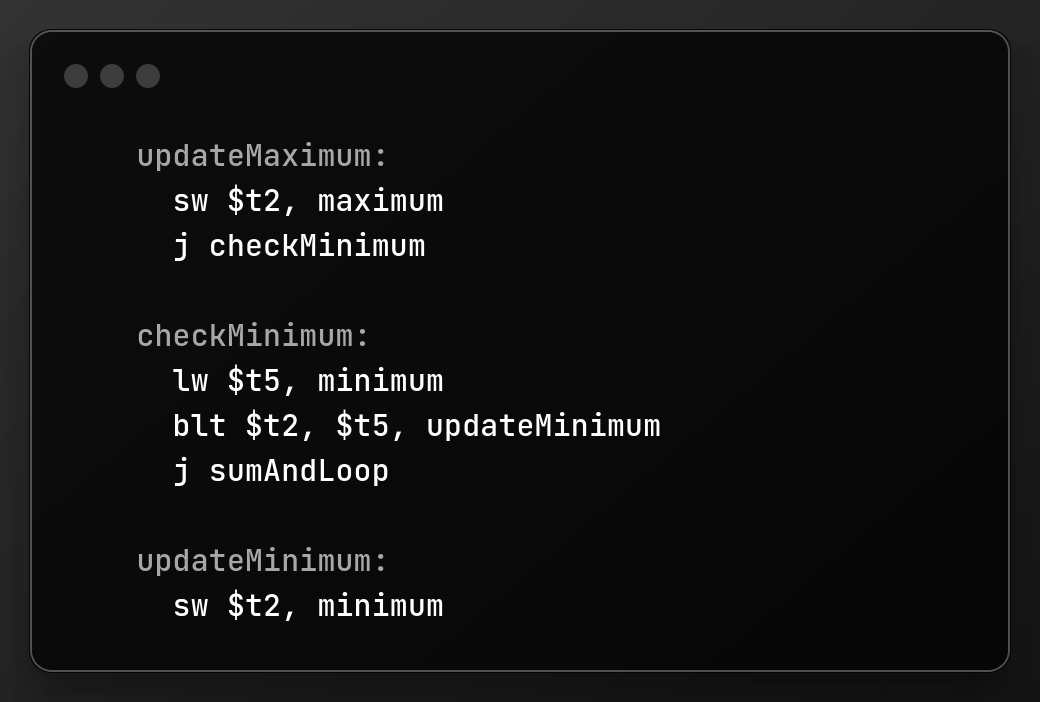
\includegraphics[scale = 0.25]{4th.png}
\end{center}

The sumAndLoop label adds up all the numbers entered by the user,
keeps track of the number of inputs and restarts the main loop.

\begin{center}
  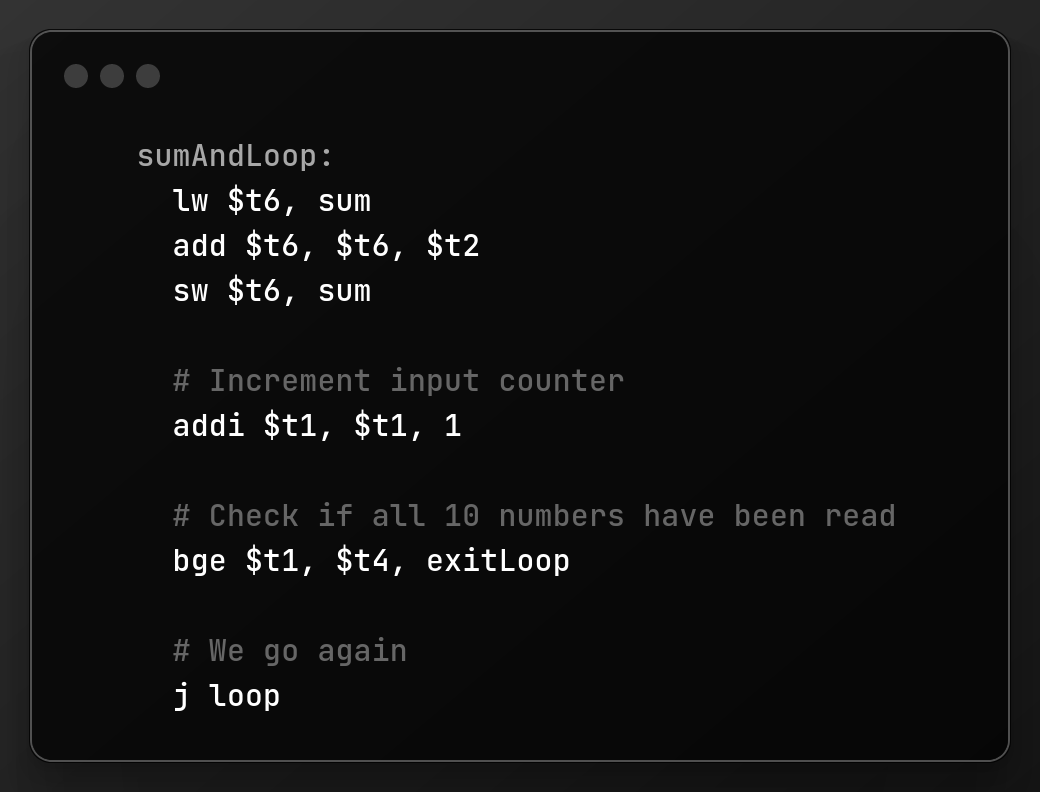
\includegraphics[scale = 0.25]{amen2.png}
\end{center}

After the loop is done, the exitLoop label will execute. It will
output the maximum, minimum and sum of the inputs entered using the 
smolprintf subprogram before exiting the program.

\begin{center}
  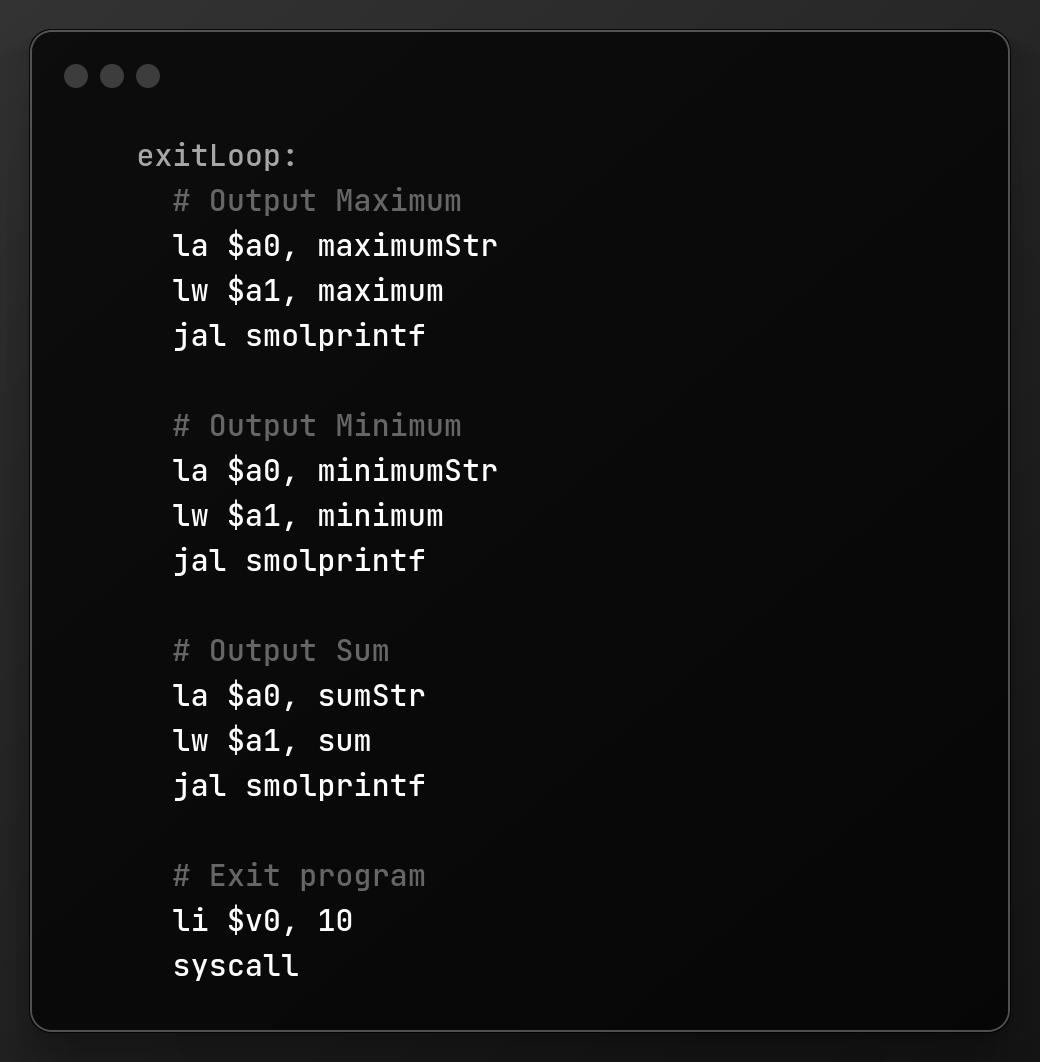
\includegraphics[scale = 0.25]{exitaaaaaaaaa.png}
\end{center}

Below is the subprogram responsible for printing the aforementioned
values. It uses the \$a0 and \$a1 registers as parameters which store
the message and value to output respectively.

\begin{center}
  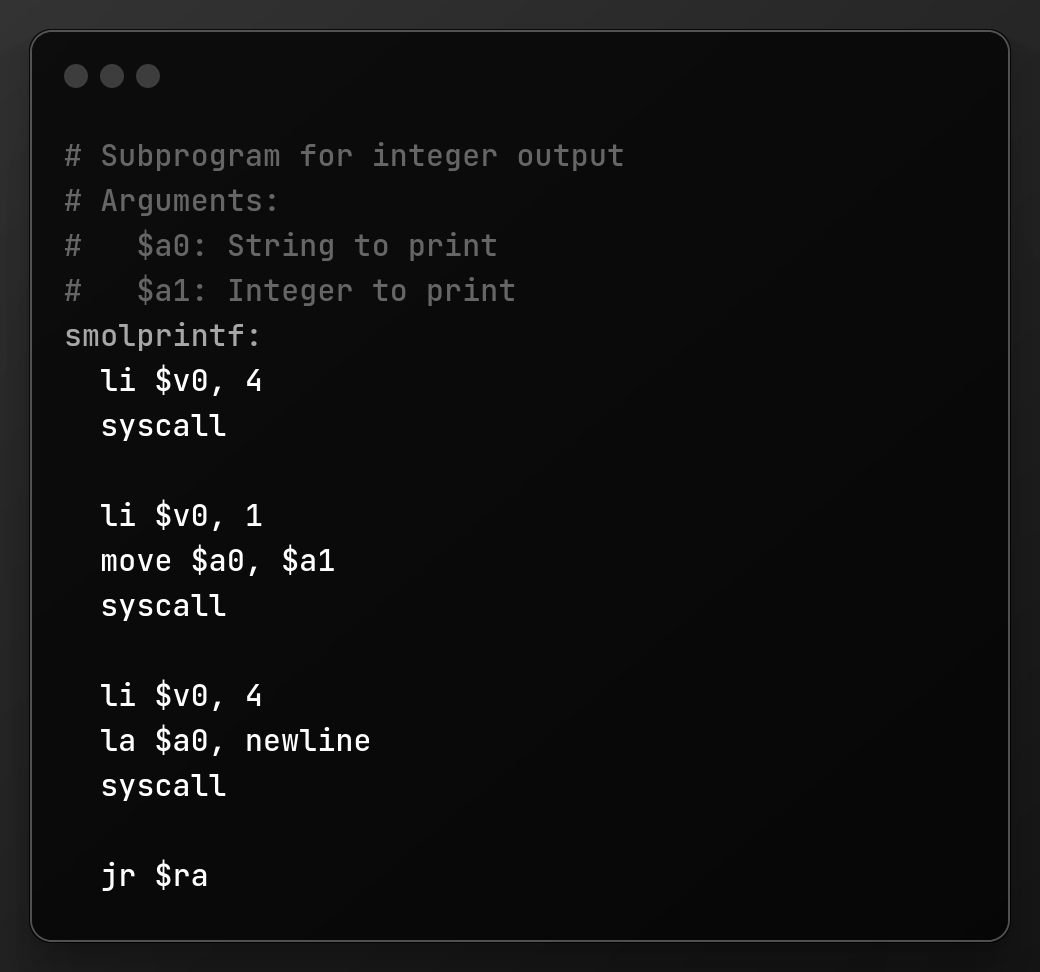
\includegraphics[scale = 0.25]{SUBBBBBB.png}
\end{center}

\section{Subprograms}
The smolprintf subprogram helped to significantly reduce the number
of lines of code. Before, to output a single line, the following was
required:

\begin{center}
  \includegraphics[scale = 0.25]{before.png}
\end{center}

The subprogram smolprintf helps to significantly reduce this by
about half:

\begin{center}
  \includegraphics[scale = 0.25]{after.png}
\end{center}

\section{Learning resources used}
\href{https://courses.missouristate.edu/kenvollmar/mars/help/syscallhelp.html}{MIPS Syscall table} 
- Syscall reference table \\
\href{https://www.youtube.com/watch?v=5AN4Fo0GiBI&t=525s}{Intro to MIPS} -
Explanation of registers and hello world program

\end{document}
